\documentclass[
25pt, 
a0paper, 
portrait, 
margin=0mm, 
innermargin=25mm,
blockverticalspace=10mm, 
colspace=10mm, 
subcolspace=8mm
]{tikzposter}

\usepackage{amssymb}
\usepackage{lipsum}
\usepackage{graphicx}
\usepackage{multicol}
\usepackage[T1]{fontenc}
%\usepackage{helvet}
\usepackage{booktabs}
\usepackage{multicol,lipsum,graphicx,float}
\usepackage[export]{adjustbox}
\usepackage{wrapfig}
\usepackage{caption}
\usepackage[labelfont=bf]{caption}

\linespread{1.1}

\definecolorpalette{bonn}{
	\definecolor{color1}{RGB}{  0, 79,159}
	\definecolor{color2}{RGB}{146,144,132}
	\definecolor{color3}{RGB}{251,185,  0}
}

\definecolorstyle{bonn}{
	\definecolor{color1}{RGB}{  0, 79,159}
	\definecolor{color2}{RGB}{146,144,132}
	\definecolor{color3}{RGB}{251,185,  0}
}
{
	\colorlet{backgroundcolor}{white}
	\colorlet{blocktitlebgcolor}{color2}
	\colorlet{blocktitlefgcolor}{black}
	\colorlet{blockbodybgcolor}{white}
	\colorlet{blockbodyfgcolor}{black}
}

\definetitlestyle{bonn}{
    width=821mm, roundedcorners=0, linewidth=0pt, innersep=8mm,
    titletotopverticalspace=80mm, titletoblockverticalspace=10mm,
    titlegraphictotitledistance=20pt
}{
    \begin{scope}
                \node[anchor=north east, inner sep=0] (uni_logo) at (412.0mm,584.5mm) {\includegraphics[height=80mm]{uni_Logo.png}};
                \draw [anchor=north east, rounded corners=50pt,line width = 6.0mm, color=color1]    (uni_logo.north east) ++(-50mm, -3.07mm) -| ++( -771mm,-1153mm);
                \draw [anchor=north east, rounded corners=50pt,line width = 6.0mm, color=color3]    (uni_logo.north east) ++( -3.08mm,-75mm) |- ++( -811mm,-1091mm);
                \draw [anchor=north east, rounded corners=50pt,line width = 6.25mm, color=color2]    (uni_logo.north east) ++(-70mm,-50.96mm) -| ++( -734.4mm, -240mm);  
    \end{scope}
}

\definelayouttheme{bonn}{
    \usecolorstyle{bonn}
    \usebackgroundstyle{Default}
    \usetitlestyle{bonn}
    \useblockstyle{Default}
    \useinnerblockstyle{Default}
    \usenotestyle{Default}
}

\usetheme{bonn}

%%%%%%%%%%%%%%% Blocks with defined height %%%%%%%%%%%%%%%%%%%%%%%%%%
\newlength\htblockbox
\newbox\blockbox

\newcommand{\mtblock}[3]{
\block{#2}{
\setlength{\htblockbox}{#1}
\parbox[t][\htblockbox][c]{\linewidth}{#3}}}

%%%%%%%%%%%%%% Sans Serif Font %%%%%%%%%%%%%%%%%%%%%%%%%%%%%%%%%%%%%%
\renewcommand{\familydefault}{\sfdefault}

\title{\Huge{\parbox{\linewidth}{\centering \textbf{Enantiomeric recognition in chiral ionic liquids: \\ Spectroscopic and structural imprints}}}}
\author{
\underline{Jan Blasius$^+$}, Paul Zaby, Oldamur Holl\'{o}czki, and Barbara Kirchner$^*$
}
\institute{
Mulliken Center for Theoretical Chemistry, Institute for Physical and Theoretical Chemistry, Beringstr. 4+6, 53115 Bonn/DE \\
%$^b$Max Planck Institute for Chemical Energy Conversion, Stiftstrasse 34--36, D-45470 Muelheim an der Ruhr
$^+$jan.blasius@thch.uni-bonn.de, $^*$kirchner@thch.uni-bonn.de
}
\tikzposterlatexaffectionproofoff

\begin{document}
\maketitle[width=\textwidth] 


\mtblock{
60mm
}{
\huge{Motivation}
}{
\large{Stereoselective synthesis of (\textit{R})- and (\textit{S})-2-butanol as well as resolution of the racemate is highly challenging. The short side chains of 2-butanol or precursor molecules with small size differences and similar chemical behaviour severely restrict the choice of asymmetric catalysts or chiral selectors. As enhanced separation or high enantiomeric excess in synthesis is usually only achieved by the attachment of further functional groups, the need for neoteric selectors is obvious for such cases in order to avoid costs and waste of additional synthetic steps. Herein we want to take a first step towards the targeted design of chiral ionic liquids (CIL) [1] selectors which are able to separate racemates of small molecules like 2-butanol without requiring prior synthetic manipulation steps.}
}

\begin{columns}
\column{0.5}


\mtblock{
170mm
}{
\huge{Model system}
}{
%\vspace{-1cm}
\begin{tikzfigure}
	\centerline{\includegraphics[trim= 0 0 0 0.7cm, width=1.03\linewidth]{./systems2.png}}
\end{tikzfigure}
\vspace{-1.5cm}
\noindent
%\begin{minipage}[c]{0.3\linewidth}
%	\begin{tikzfigure}
%		\hspace{-1.6cm}
%		\includegraphics[trim= 0 0 0 13cm, width=.8\linewidth]{./ion_pair.png}
%	\end{tikzfigure}
%\end{minipage}
%\begin{minipage}[c]{0.69\linewidth}
	\large{Our model system is composed of 1 \textbf{(\textit{R})} or \textbf{(\textit{S})-2-butanol} molecule dissolved in 10 ion pairs of the chiral ionic liquid \textbf{1-ethyl-3-methylimidazolium (\textit{L})-alaninate.} It has been shown that the achiral cation is prone for symmetry breaking due to the presence of the chiral anion. [2,3] This induced chirality amplifies the asymmetry within the liquid, which may have significant effects on the solvation of chiral compounds in this CIL.}
%\end{minipage}
}

\mtblock{
225mm
}{
\huge{Spectroscopic imprint}
}{
\noindent
\begin{minipage}[c]{0.68\linewidth}
	\begin{tikzfigure}
		\centerline{\includegraphics[trim= 0.5cm 0 0 0,width=.99\linewidth]{./vcd.pdf}}
	\end{tikzfigure}
\end{minipage}
\begin{minipage}[c]{0.31\linewidth}
\vspace{-2cm}
\Large{\textbf{VCD spectra}} \\[1.3ex] \large{VCD measures the different attenuation of left- and right-circularly polarized infrared radiation and provides three-dimensional structural information of chiral molecules. [4,5]}
\end{minipage}

\vspace{-0.5cm}
\large{The global spectrum is dominated by contributions from the chiral anion and does not reveal any information about chiral discrimination. However, the achiral cation features mirror-imaged VCD spectra, illustrating a symmetry breaking of its achiral structure. [2,3] Additionally both 2-butanol enantiomers do not show exact mirror-imaged VCD spectra as it is actually known for the neat bulk phase, [6] implying different conformational preferences for the (\textit{R})- and (\textit{S})-enantiomers in the CIL.}

}

\mtblock{
70mm
}{
\huge{Acknowledgement}
}{\vspace{2.8cm}\large{The authors thank the DFG for financial support.}
\vspace{1cm}
\begin{multicols}{2}
		\begin{tikzfigure}
			\includegraphics[trim= -0.5cm 0 0 0,width=\linewidth]{dfg_logo.pdf}
			\includegraphics[trim= -1cm 0 0 6cm,width=\linewidth]{travis_logo.pdf}
		\end{tikzfigure}
\end{multicols}
}

\mtblock{
93mm
}{
\huge{References}
}{

[1] P. S. Schulz, N. M\"uller, A. B\"osmann, P. Wasserscheid, Angew. Chem. Int. Ed. \textbf{2007}, 46, 1293-1295. [2] P. Oulevey, S. Luber, B. Varnholt, T. B\"urgi, Angew. Chem. Int. Ed. \textbf{2016}, 55, 11787-11790. [3] J. Blasius, R. Elfgen, O. Holl\'{o}czki, B. Kirchner, Phys. Chem. Chem. Phys. \textbf{2020}, 22, 10726-10737. [4] J. Blasius, B. Kirchner, J. Phys. Chem. B \textbf{2020}, 124, 7272-7283. [5] B. Kirchner, J. Blasius, L. Esser, W. Reckien, Adv. Theory Simul. \textbf{2021}, 4, 2000223. [6] M. Thomas, B. Kirchner, J. Phys. Chem. Lett. \textbf{2016}, 7, 509-513.

}

\column{0.5}

\mtblock{
615mm
}{
\huge{Conformational imprint}
}{
\vspace{-0.5cm}
\noindent
\begin{minipage}[c]{0.66\linewidth}
	\begin{tikzfigure}
		\centerline{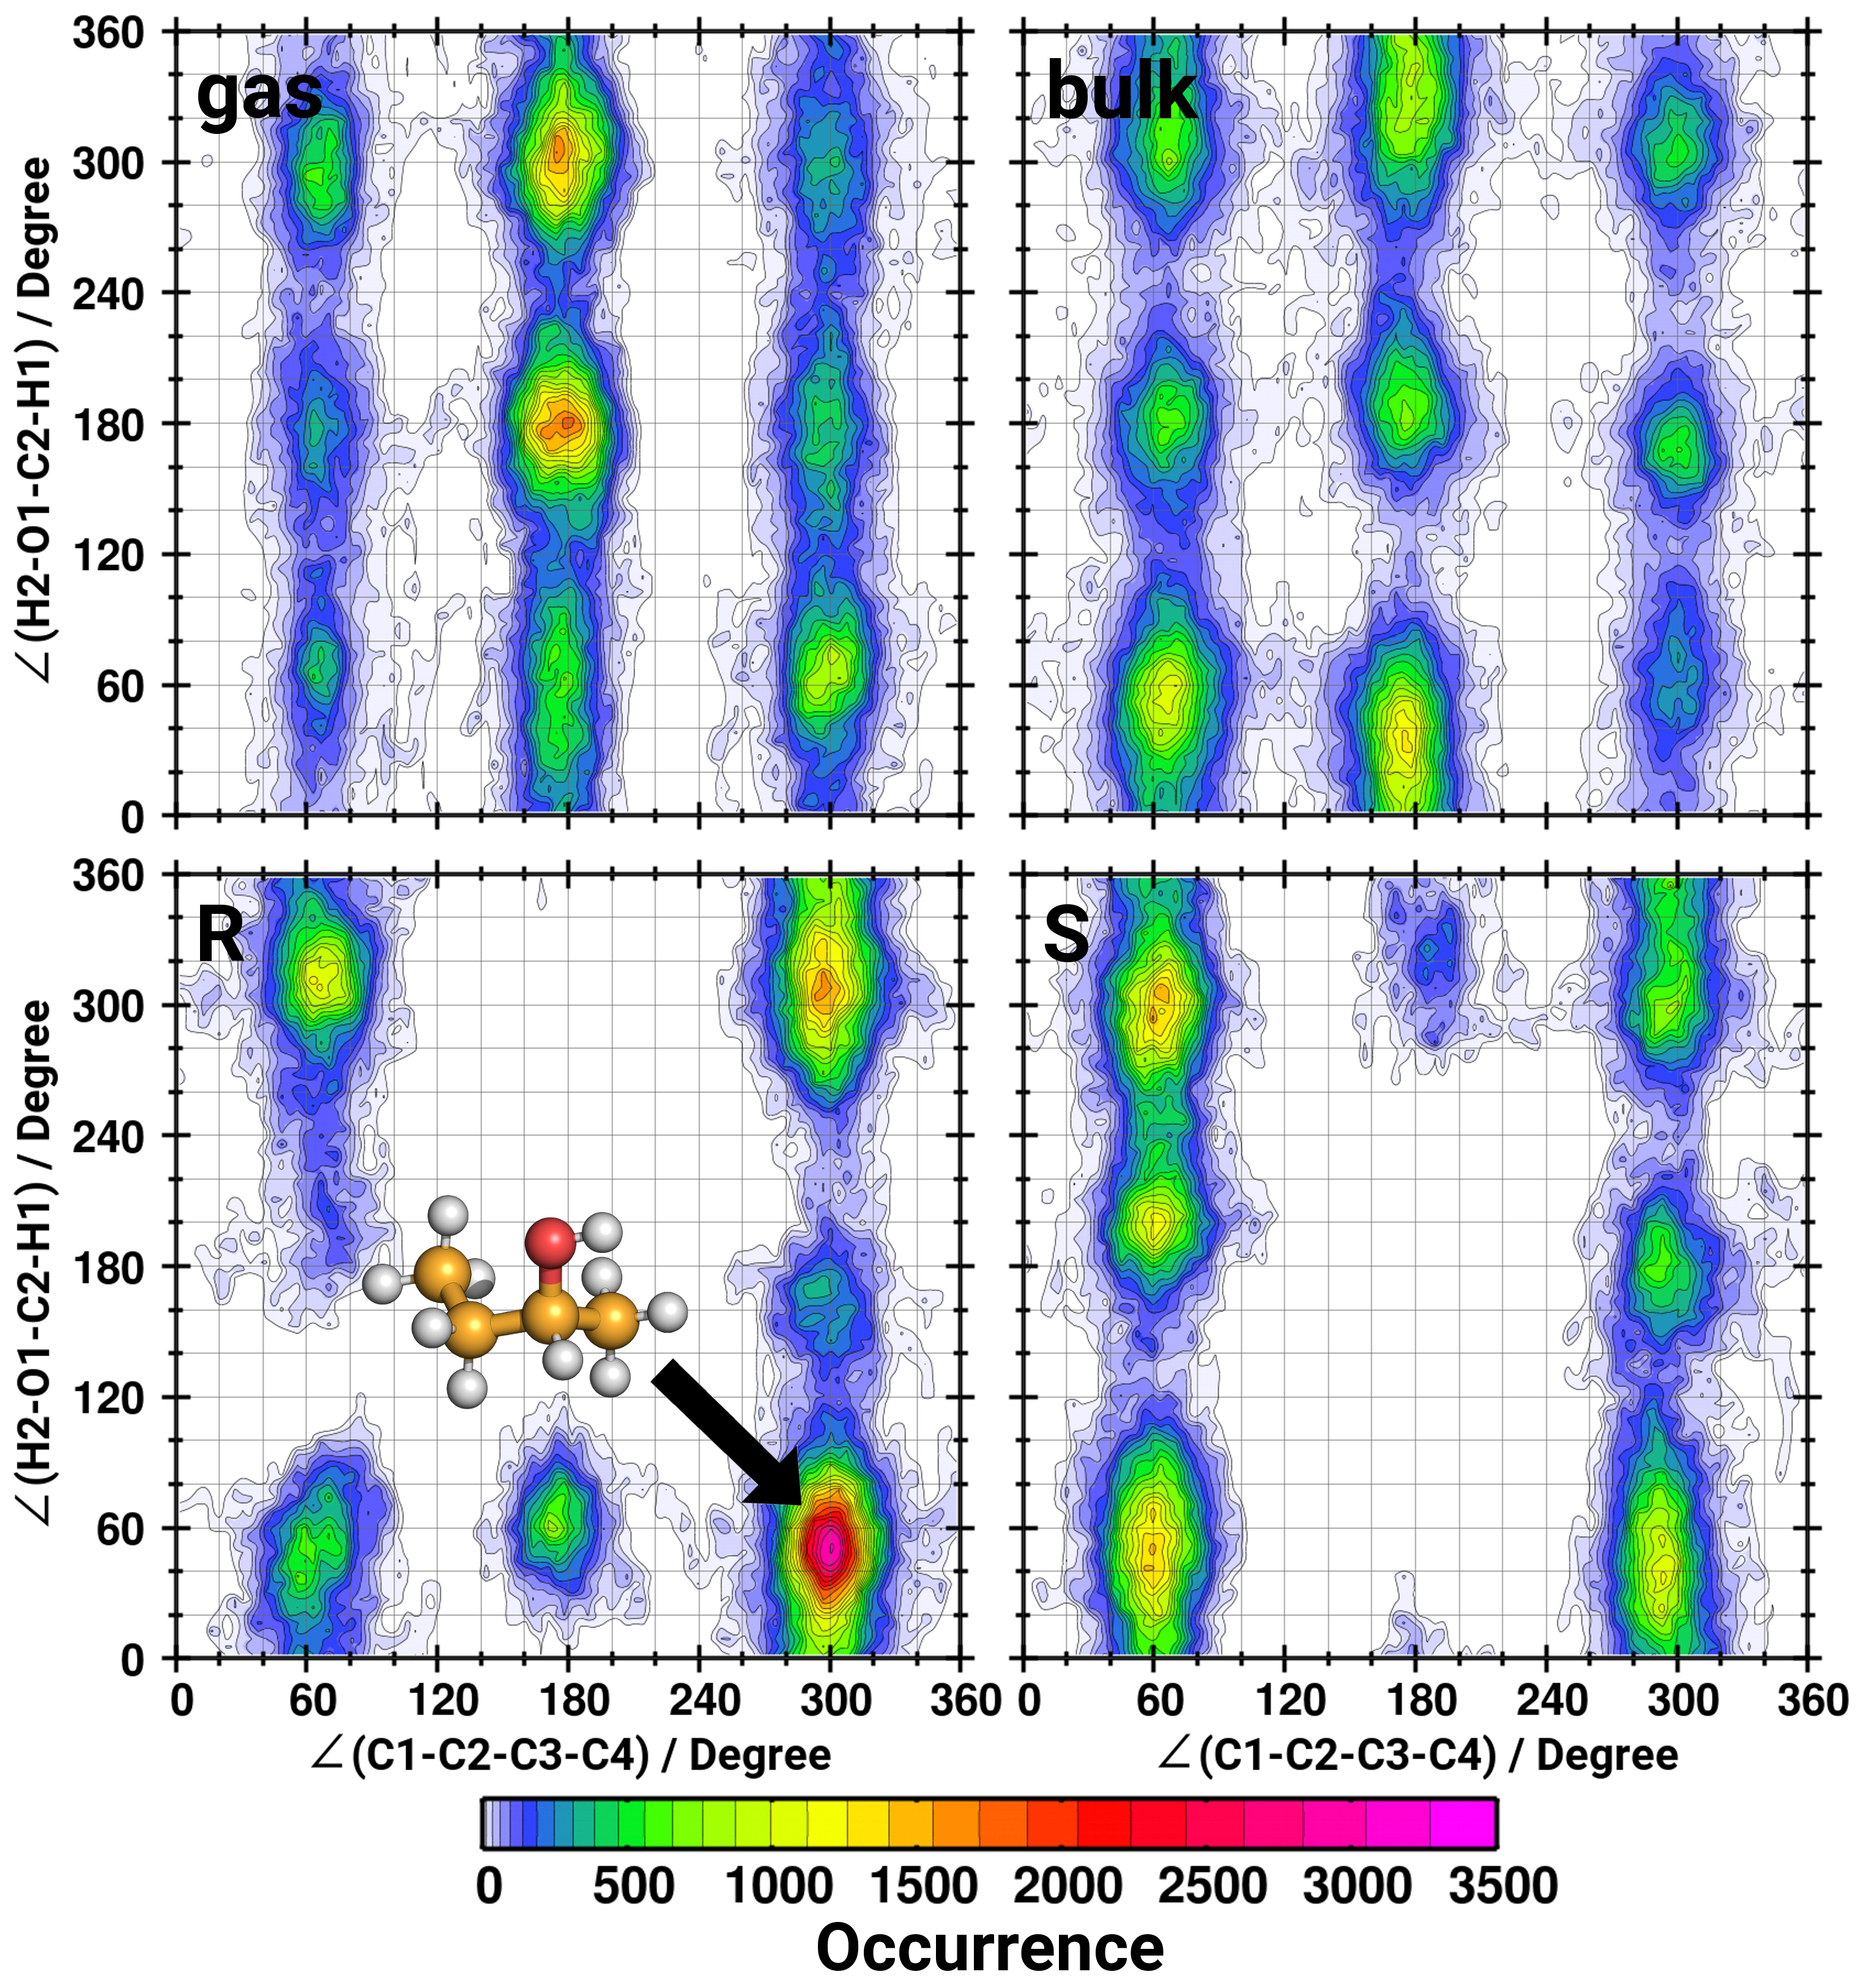
\includegraphics[trim= 1.9cm 0 0 0,width=.88\linewidth]{./but_cdf.png}}
	\end{tikzfigure}
\end{minipage}
\begin{minipage}[c]{0.33\linewidth}
%\vspace{-7cm}
\Large{\textbf{Conformer plots}} \\[1.3ex] \large{Correlate the dihedral angles $\angle$(C1-C2-C3-C4) and $\angle$(H2-O1-C2-H1) in order to access information about the occurrence of each conformer.}
\vspace{2.5cm}
	\begin{tikzfigure}
		\centerline{\includegraphics[width=.8\linewidth]{./butanol.png}}
	\end{tikzfigure}
\end{minipage}

\vspace{-1cm}
\large{In system \textbf{R} one conformation is conspicuously dominant (39\%) compared to its mirror-imaged counterpart in system \textbf{S} (23\%). Thus, 2-butanol adapts specific structures in order to fit best to the binding partners within the solvent. The efficiency of this induced fit is different for the two enantiomers, as shown by the difference in the averaged electronic energies: System \textbf{R} is stabilized by $\Delta$E = 18.8 kJ/mol compared to system \textbf{S}.}

\begin{minipage}[c]{0.66\linewidth}
	\begin{tikzfigure}
		\centerline{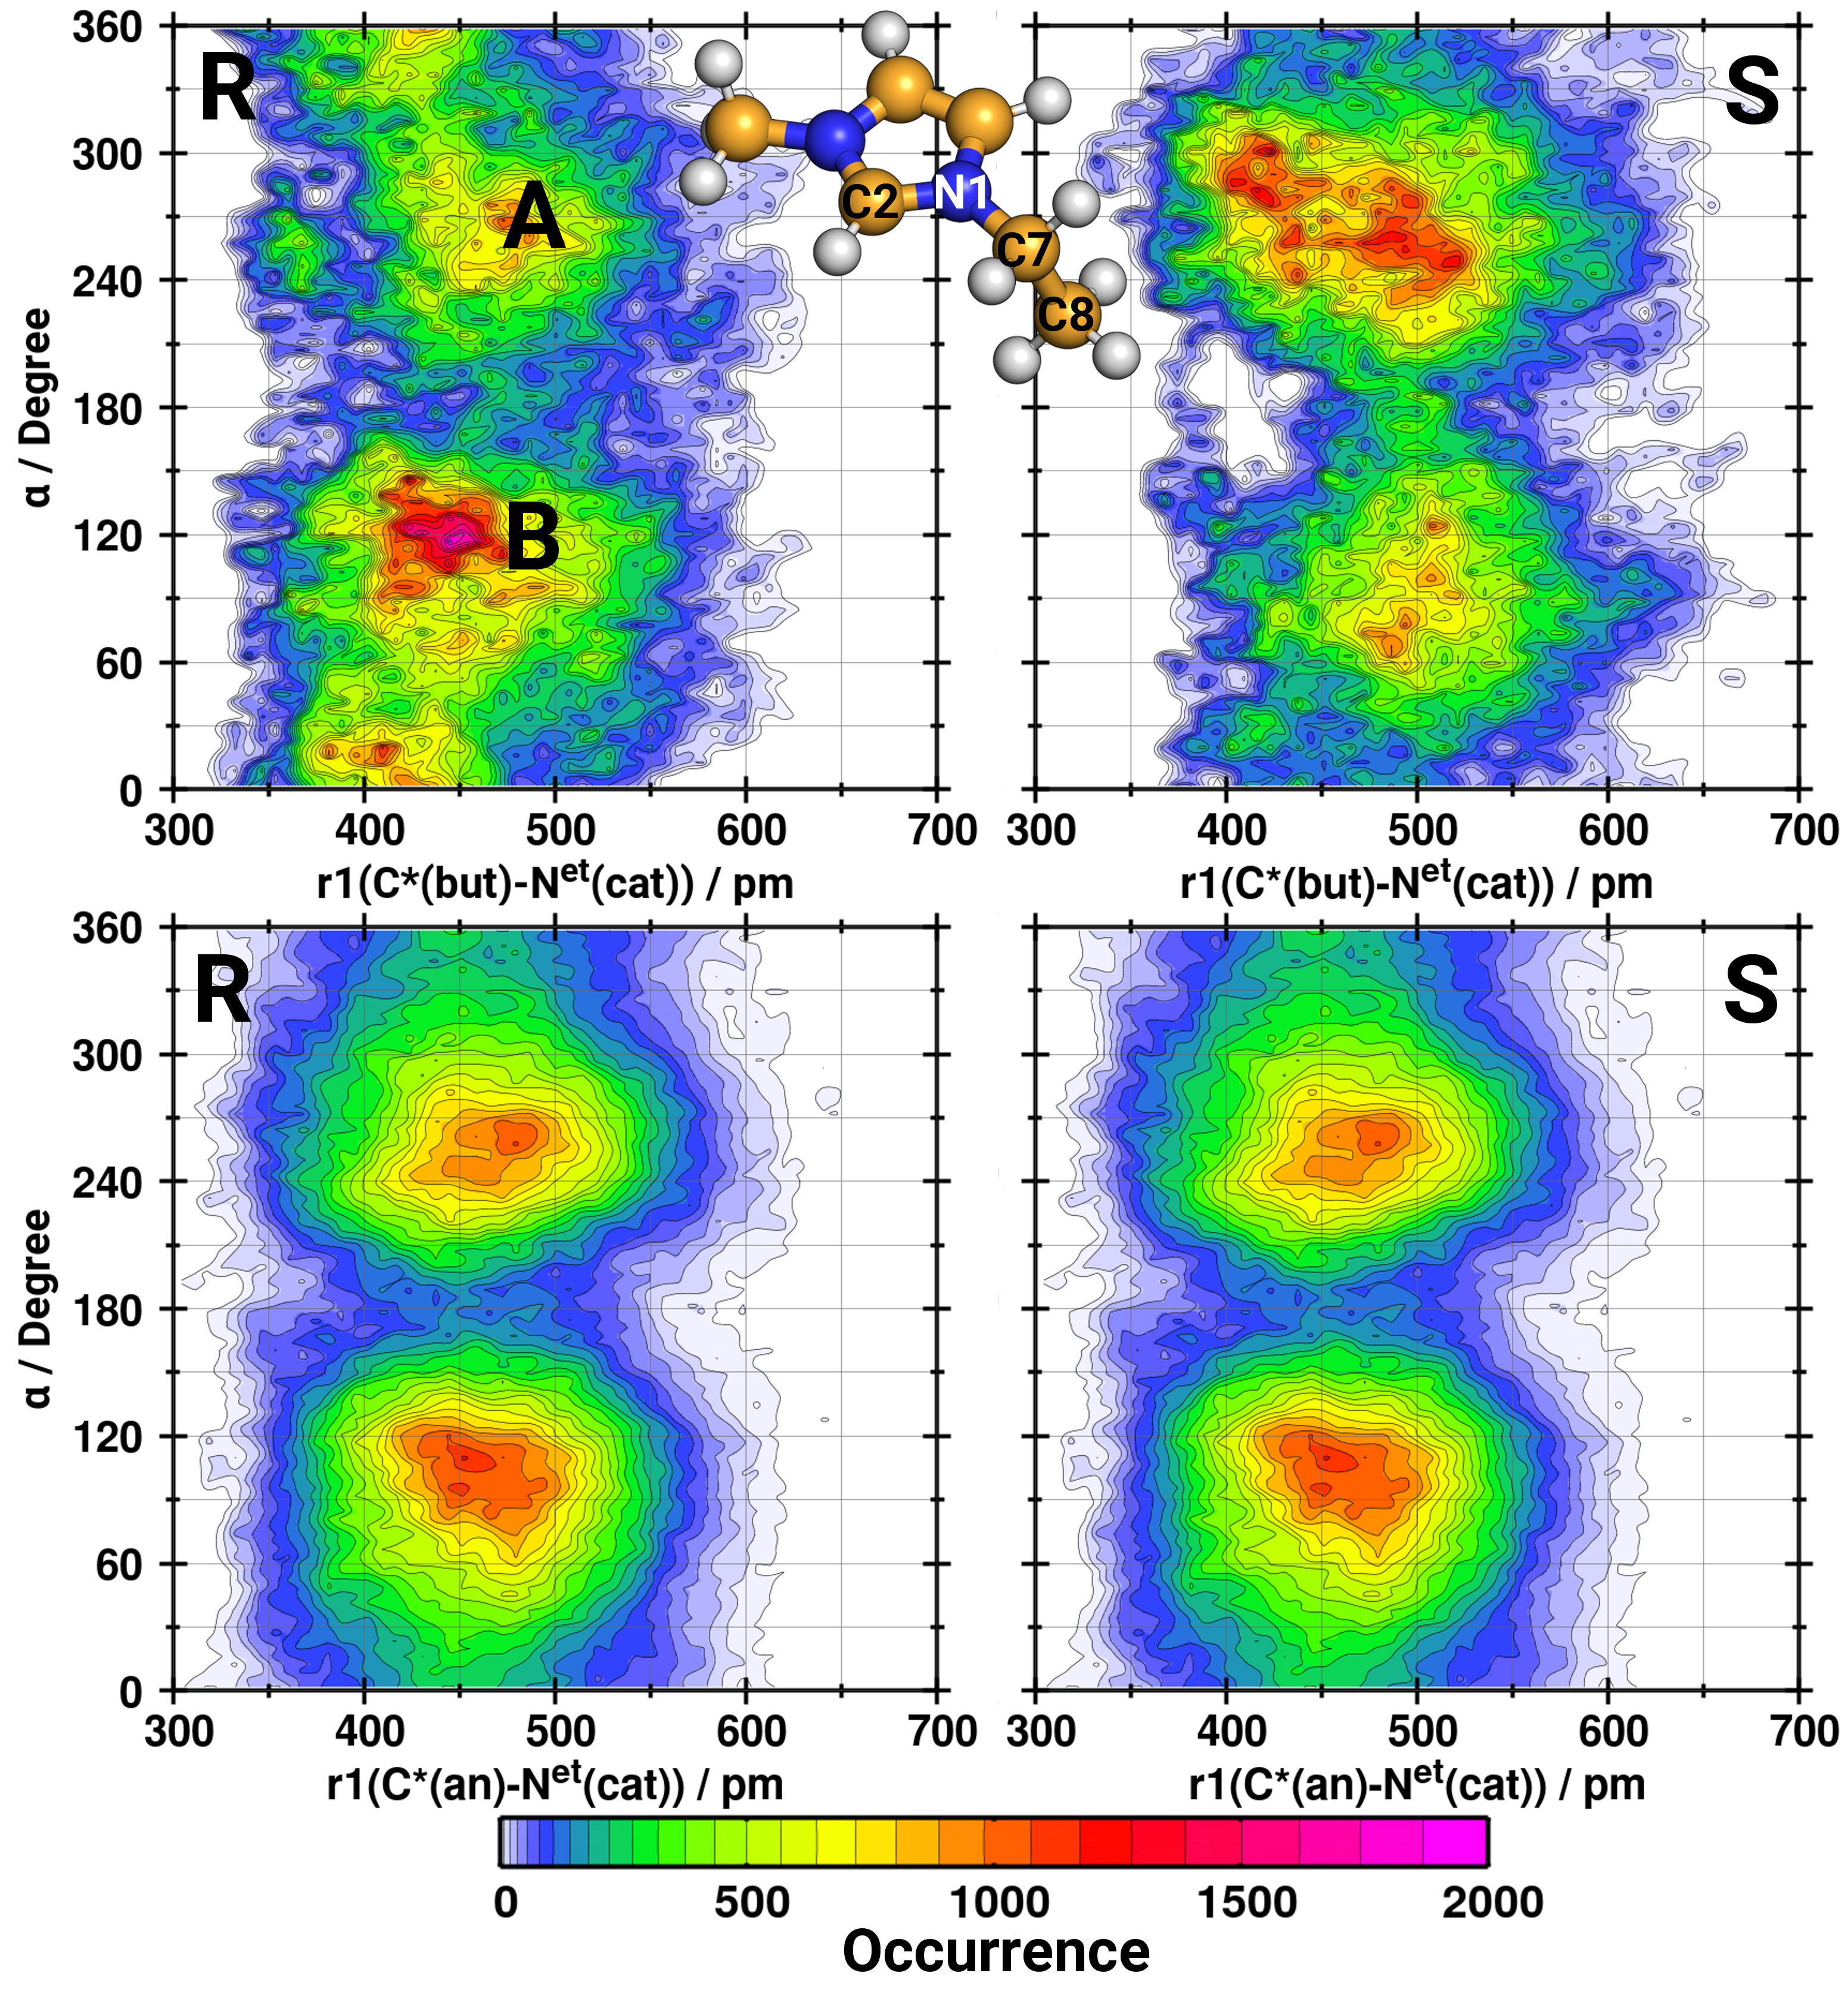
\includegraphics[trim= 1.9cm 0 0 0,width=.88\linewidth]{./cat_cdf.png}}
	\end{tikzfigure}
\end{minipage}
\begin{minipage}[c]{0.33\linewidth}
%\vspace{-7cm}
\Large{\textbf{Conformer plots}} \\[1.3ex] \large{Correlate the dihedral angle $\alpha$(C2-N1-C7-C8) and the distance between 2-butanol (top) or anion (bottom) and its closest cation.}
\vspace{2.5cm}
	\begin{tikzfigure}
		\centerline{\includegraphics[trim= 5cm 0 0 0, width=1.1\linewidth]{./cation_mirror.png}}
	\end{tikzfigure}
\end{minipage}

\vspace{-1cm}
\large{Chiral induction induces a distorted equilibrium of the ethyl group rotation. The interaction of the chiral anion with the cation has this very effect, enriching conformation \textbf{B}. While (\textit{R})-2-butanol also induces conformation \textbf{B}, (\textit{S})-2-butanol induces structures with opposite chirality, i.e. conformation \textbf{A}. Thus, while (\textit{R})-2-butanol fits well into the environment created by the anion, (\textit{S})-2-butanol competes with the anion for enforcing opposite conformations on the cation.}

}



\mtblock{
72mm
}{
\huge{Conclusion and next steps}
}{
\large{Chiral discrimination between 2-butanol enantiomers originates from asymmetrization of the ethyl group rotation of the cation being opposite around both enantiomers. The asymmetrization effects by anion and solute are conflicting in the homochiral (\textbf{S}) and harmonious in the heterochiral (\textbf{R}) system. As next steps, novel CIL selectors with permanently chiral cations resembling the structures imprinted by the respective solute will be designed.}
}




\end{columns}

\end{document}
